\documentclass[11pt, oneside]{article} 
\usepackage{geometry}
\geometry{letterpaper} 
\usepackage{graphicx}
	
\usepackage{amssymb}
\usepackage{amsmath}
\usepackage{parskip}
\usepackage{color}
\usepackage{hyperref}

\graphicspath{{/Users/telliott_admin/Tex/png/}}
% \begin{center} 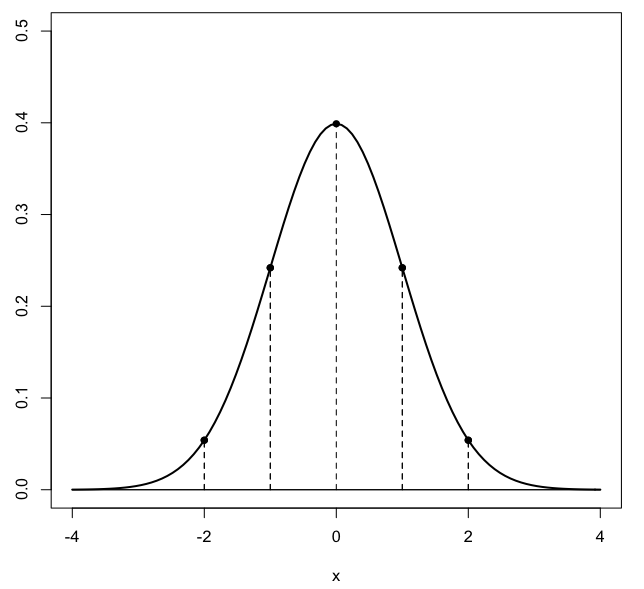
\includegraphics [scale=0.4] {gauss3.png} \end{center}

\title{Introduction}
\date{}

\begin{document}
\maketitle
\Large

In this chapter we review briefly the most common integrals.  Additional depth is given in a later chapter on \hyperref[sec:Techniques_of_integration]{\textbf{Techniques of integration}}.

\subsection*{powers of x}
The first \textbf{differentiation} that is done in basic calculus is
\[ \frac{d}{dx} (x^n) = [x^n]' = n x^{n-1} \]
This answer is correct regardless of whether $n$ is positive or negative, an integer or a rational number, or even irrational. 

The proof for positive integers $n \in \{ 2, 3 \}$ is simple.  A general proof for positive integers is fairly easy using the binomial theorem.  

Implicit differentiation will give a simple proof for all rational exponents.  Still later we will have a proof for all real numbers.  See \hyperref[sec:Implicit_differentiation]{\textbf{here}}.  We will finally find a function that yields $x^{-1}$ as its derivative when we talk about the natural logarithm.
 
Ignoring some subtleties, we can \textbf{integrate} by reversing the process.  We write 
\[  x^n = \int n x^{n-1} \ dx \]

A real math book will tell you that when the formula stands alone like this, we should add a constant of integration:  $x^n + C$.  But we are mostly using integrals to calculate areas and volumes, which means we determine the value of a definite integral by computing the difference of two expressions which both contain $C$, so it cancels.  

If the factor of $n$ is not given in the problem, we insert it as a divisor up front:
\[  \int x^{n-1} \ dx = \frac{1}{n} x^n \]
\[  \int x^{n} \ dx = \frac{x^{n+1} }{n+1} \]
 
\[ \int \sqrt{x} \ dx = \frac{2}{3} x^{3/2} \]
\[ \int \frac{1}{\sqrt{x}} = 2 \sqrt{x} \]

A common convention for notation is that $\int f(x) = F(x)$.  Or, the other way around $f(x)$ is the derivative of $F(x)$, so $f(x) = F'(x)$.  Let's make a table.

\[ \begin{matrix} f(x) \ \ \ \ \ & F(x) \\
& \\
1 \ \ \ \ \ & x \\
x \ \ \ \ \ & x^2/2 \\
x^2 \ \ \ \ \ & x^3/3 \\
x^n \ \ \ \ \ & x^{n+1}/n+1 \\
\frac{1}{\sqrt{x}}  \ \ \ \ \ & 2 \sqrt{x} \\
\sqrt{x}   \ \ \ \ \ & \frac{2}{3} x^{3/2}  \\
& \\
\cos x  \ \ \ \ \ & \ \ \sin x \\
\sin x  \ \ \ \ \ & - \cos x \\
& \\
e^{x} \ \ \ \ \ & e^{x} \\
1/x \ \ \ \ \ & \ln x \\
& \\
a \cos ax \ \ \ \ \ & \sin ax \\
\cos ax \ \ \ \ \ & \frac{1}{a} \ \sin ax \\
& \\
ae^{ax}  \ \ \ \ \ & \ \ e^{ax} \\
e^{ax}   \ \ \ \ \ & \frac{1}{a} \ e^{ax} \\
\end{matrix} \]

We will look at proofs for these trig functions and the exponential and logarithm in some detail in the next few chapters.  For now, let's accept them provisionally.

\subsection*{fractional powers}

Two additional integrals that we here add come from differentiations as seen in the chapter on the chain rule.  With $a^2$ a constant:
\[ \frac{d}{dx} \sqrt{a^2 - x^2} =  - x \ \frac{1}{\sqrt{a^2 - x^2}} \]
\[ \frac{d}{dx} (a^2 - x^2)^{3/2} = -3x \ \sqrt{a^2 - x^2} \]

To integrate, we reverse directions.  The first one is
\[ \int x \ \frac{1}{\sqrt{a^2 - x^2}} \ dx = - \ \sqrt{a^2 - x^2} \]
To check this, do the differentiation.  The factor of $1/2$ on the right-hand side from the power and the leading $-1$ are canceled by the factor of $-2$ from the chain rule.  Those are easy.  The important thing is that we have that $x$ under the integral sign.

The second one is
\[ \int 2x \ \sqrt{a^2 - x^2} \ dx = - \frac{2}{3} \ (a^2 - x^2)^{3/2} \]
Again, check by differentiating the right-hand side.  We get a factor of $3/2$ from the power, which cancels the leading $2/3$, then we get $-2x$ from the chain rule and cancel the minus sign.  Factors of $2$ and minus signs are easy, but we must have that $x$ on the left, otherwise the answer will be much different.

\subsection*{square root}

We will show that the integral of the square root gives the correct answer.  Suppose we plot
\[ y = \sqrt{x} \] over the interval $[0,1]$.  The area under this curve is the shaded region.
\begin{center} 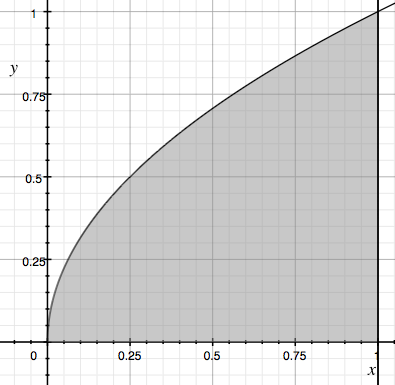
\includegraphics [scale=0.4] {sqrt_shaded.png} \end{center}

The area seems to be more than $1/2$, but how much more?  Now, take the very same plot, flip it over and rotate 90 degrees.  We obtain something that is more familiar, namely the plot of $y = x^2$.  The area under this curve is the white region
\begin{center} 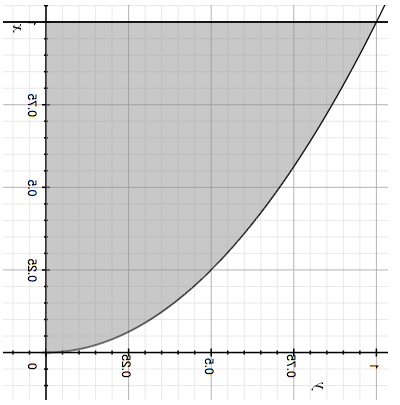
\includegraphics [scale=0.4] {sqrt_shaded_rotate.png} \end{center}

Clearly 
\[ \int_0^1 \sqrt{x} \ dx + \int_0^1 x^2 \ dx = 1 \]
If you look in the list of formulas above (or just calculate) you will find that the first integral is equal to $2/3$ and the second one is equal to $1/3$.

This result holds for other intervals, not just $[0,1]$.

Let's integrate to find the area under the curve in the interval $[0,b^2]$ (shaded gray below).  We use $b^2$ for reasons that will be obvious in a minute.
\[ A = \int_0^{b^2} \sqrt{x} \ dx = \frac{2}{3} x^{3/2} \ \bigg |_0^{b^2} = \frac{2}{3} b^3  \]

\begin{center} 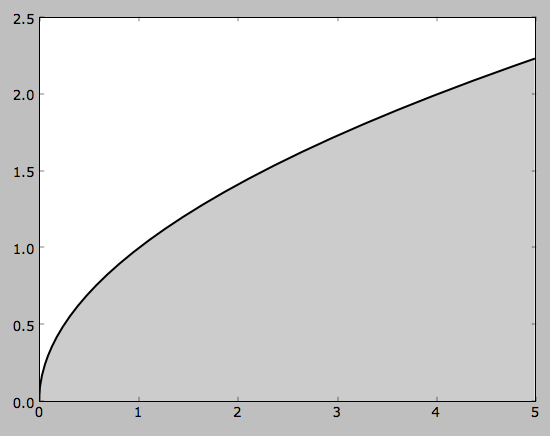
\includegraphics [scale=0.3] {square_root_plot.png} \end{center}

Now, consider $x$ as a function of $y$:
\[ x = y^2 \]

Integrate to find the area between the curve and the $y$-axis (shaded white above).  The only trick is that the bounds are $[0,b]$ because we want to add the two areas together to form a rectangle and the point on the curve at the upper bound will be $x = b^2, y = b$.
\[ \int_0^{b} y^2\ dy = \frac{1}{3} y^3 \ \bigg |_0^{b} = \frac{b^3}{3}  \]

Adding the results together, we obtain $b^3$ as the area of a box with width $\Delta x = b^2$ and height $\Delta y = b$, which is correct.

\subsection*{reversing the product rule}

Playing around with the product rule can lead to the discovery of other important integrals that we will encounter later.  The most important is
\[ (\sin x \cos x)' = \cos x \cos x - \sin x \sin x  \]
\[ = \cos^2 x - \sin^2 x \]

Recall the most basic trig identity:
\[ \sin^2 x + \cos^2 x = 1 \]
\[ -\sin^2 x = \cos^2 x - 1 \]
so
\[ (\sin x \cos x)' = 2 \cos^2 x - 1 \]
integrating
\[ \sin x \cos x = 2 \int \cos^2 x \ dx  - x \]
\[ \int \cos^2 x \ dx = \frac{1}{2} (x + \sin x \cos x) \]
That is one we'll want to remember.  We will use several techniques of integration to derive it from first principles, but this is the easiest way.  See \hyperref[sec:Cosine_squared]{\textbf{here}}.

Here are a few others:
\[ (x \ln x)' = \ln x + \frac{x}{x} = \ln x + 1 \]
\[ \int \ln x \ dx = x \ln x - x \]

\[ (x^2 \ln x)' = 2 x \ln x + x \]
\[ \int 2 x \ln x = x^2 \ln x - \frac{x^2}{2} \]

\[ (x e^x)' = e^x + x e^x \]
\[ \int x e^x \ dx = x e^x - e^x \]

\subsection*{Stirling's approximation}
For an application, consider
\[ \int \ln x \ dx = x \ln x - x \]

Computing $n!$ gets unwieldy for large $n$ (at least, without computers).  It comes up in probability and other places.  There is a famous formula for $n!$ called Stirling's approximation which comes in a more precise version
\[ n! \approx \sqrt{2 \pi n} \ (\frac{n}{e})^n \]
and a less precise one
\[ \ln n! \approx n \ln n - n \]

The latter is easily derived:
\[ \ln n! = \ln 1 + \ln 2 + \dots \ln n \]
\[ = \sum_{k=1}^n \ln k \]
\[ \approx \int_1^n \ln x \ dx \]
which we showed is
\[ = x \ln x - x \ \bigg |_1^n \]
\[ = (n \ln n - n) - (1 \ln 1 - 1) \]
\[ = n \ln n - n + 1 \]
\[ \approx n \ln n - n  \]


\end{document}